\begin{figure}[htbp]
\centering
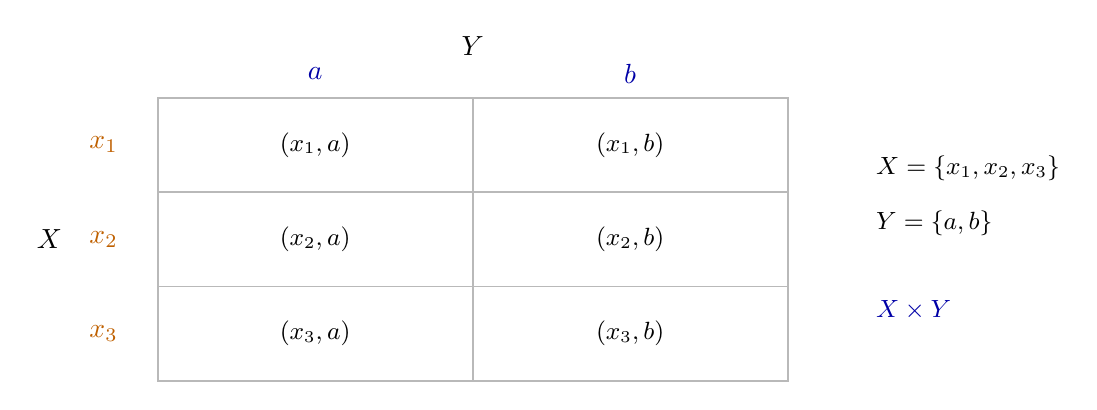
\begin{tikzpicture}[x=1.25cm,y=1cm,font=\small]
    \draw[gray!55,line width=0.7pt] (2,0) rectangle (8.4,3.6);
    \draw[gray!55,line width=0.7pt] (5.2,0) -- (5.2,3.6);
    \draw[gray!55,line width=0.7pt] (2,1.2) -- (8.4,1.2);
    \draw[gray!55,line width=0.7pt] (2,2.4) -- (8.4,2.4);
    \node[font=\bfseries] at (5.2,4.25) {$Y$};
    \node[font=\bfseries] at (0.9,1.8) {$X$};
    \node[blue!65!black,font=\bfseries] at (3.6,3.9) {$a$};
    \node[blue!65!black,font=\bfseries] at (6.8,3.9) {$b$};
    \node[orange!75!black,font=\bfseries] at (1.45,3.0) {$x_1$};
    \node[orange!75!black,font=\bfseries] at (1.45,1.8) {$x_2$};
    \node[orange!75!black,font=\bfseries] at (1.45,0.6) {$x_3$};
    \foreach \x/\y/\first/\second in {3.6/3.0/x_1/a,6.8/3.0/x_1/b,3.6/1.8/x_2/a,6.8/1.8/x_2/b,3.6/0.6/x_3/a,6.8/0.6/x_3/b} {
        \node at (\x,\y) {$(\first,\second)$};
    }
    \node[anchor=west,font=\small] at (9.2,2.7) {$X=\{x_1,x_2,x_3\}$};
    \node[anchor=west,font=\small] at (9.2,2.0) {$Y=\{a,b\}$};
    \node[anchor=west,font=\small\bfseries,text=blue!65!black] at (9.2,0.9) {$X\times Y$};
\end{tikzpicture}
\caption{The Cartesian product is a complete grid of ordered pairs: rows choose the first coordinate and columns choose the second.}
\label{fig:cartesian-product-grid}
\end{figure}